\chapter{Catching Attackers in Restricted Network Areas}
\label{chap:concept}

Zoning a network is often well-known method to restrict 

\section{Introduction}

Honeypots that are accessible via the Internet do receive a broad range of attacks.
As \citet{Spitzner2003} noted, a honeypot is not strictly bound to run in a \ac{dmz} or a network with direct Internet access.
Moreover, the correct location has to be chosen based on the goals of the honeypots.
For example, one goal is to catch attackers behind a perimeter firewall to reveal leaks or vulnerabilities.
Beforehand, our honeypot was broadly available on the Internet, and attackers could probe it easily.
It collected on average $\numprint{55000}$ attacks per day, resulting in a total amount of $\numprint{786564}$ attacks.
This amount sounds reasonable when no perimeter firewall secures the server.
Heidelberg University works ...% zoning
An interesting question is if attackers have access to restricted zones at the Heidelberg University.
It arises during the research of T-Pot if an adversary would try to probe any hosts in the internal University network.
In order to detect such events we present the Heidelberg Connection Acceptance Tool that helps to identify any threats in a network.
In addition, it offers to deploy multiple instance and collect their data in a centralized instance. 

\section{Heidelberg Connection Acceptance Tool}

The acronym MADCAT stands for Mass Attack Detection Connection Acceptance Tools.

It works as a honeypot-like detection application with low interaction level. 
Its key idea is to log every connection attempt and further process it to retrieve credentials, or shell exploitation.
\autoref{fig:madcat-architecture} gives an inside how MADCAT works.
It runs on an Ubuntu distribution either $18.04$ or $20.04$.
We have tested it on Ubuntu $18.04$.
It processes packets from any interface that has been configured.
As an example, we could process Ethernet and wireless packets.
MADCAT itself consists of six independent modules that communicating with each other through a pipeline.
Respectively, for TCP, UDP, ICMP, and RAW packets it provides a module for it.
A module is responsible for analyzing packets and logging the results in a queue.
In addition, UDP and TCP offers proxies to tunnel to packets to a service.
TCP postprocessor reads in a 5 seconds interval the newly arrived TCP packets and processes them accordingly.
It resolves packets to log data including source IP address, protocol and event type.
The enrichment processor is the final process step.
Its purpose is to log all written packets of the queue in a specified format for further analyzation.
The key idea of MADCAT is to get an inside if attackers have access to a certain network.
In contrast to T-Pot, we do not want to know what specific attacks are operated on our honeypot.
Instead, we do want to ensure that no one else than authorized users have access.
Especially in high confidential areas, no attacker should be capable of sending even a single packet to a host in the network.
Tracking packets on a detailed level is not provided by the vast range of honeypots.

\begin{figure}[ht]
    \centering
    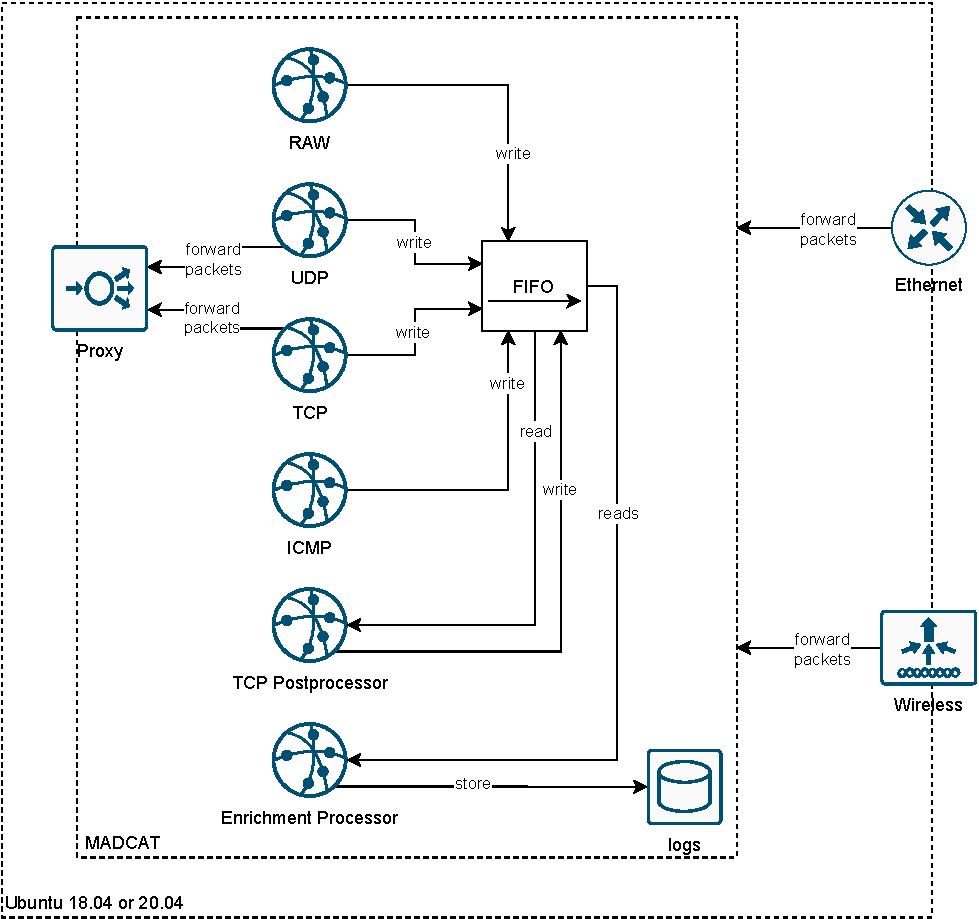
\includegraphics[width=\textwidth]{figures/heicat-architecture.pdf}
    \caption[MADCAT architecture]{MADCAT architecture. The Ethernet and wireless interface forwards the respective packets to the desired module.}
    \label{fig:madcat-architecture}
\end{figure}

The question of how secure the internal University network is arose during the deployment of T-Pot.
At the University, the network splits into different zones.
We decided to focus on the $219$-zone that is similar to a restricted zone.
This zone is specified by the subnet \ipAddress{129.206.219.0/24}.
In this zone 
Respectively, our host machine is located with the that network with \ipAddress{129.206.219.88}

Our goal is to catch any connection attempt that has been made to our honeypot.
\autoref{fig:heicat-concept} carries out our concept.
Our concept is divided into to hosts.
The first one is responsible for providing Kibana, and Elasticsearch to crawl through logs.
The honeypot consists of MADCAT in conjunction with P0f, Suricata, and FATT for additional information.
Like T-Pot, we use Logstash to forward our data to Elasticsearch.
One benefit is the centralized approach to store data.
It allows to randomly deploy more instances to collect data from other zones.

\begin{figure}[ht]
    \centering
    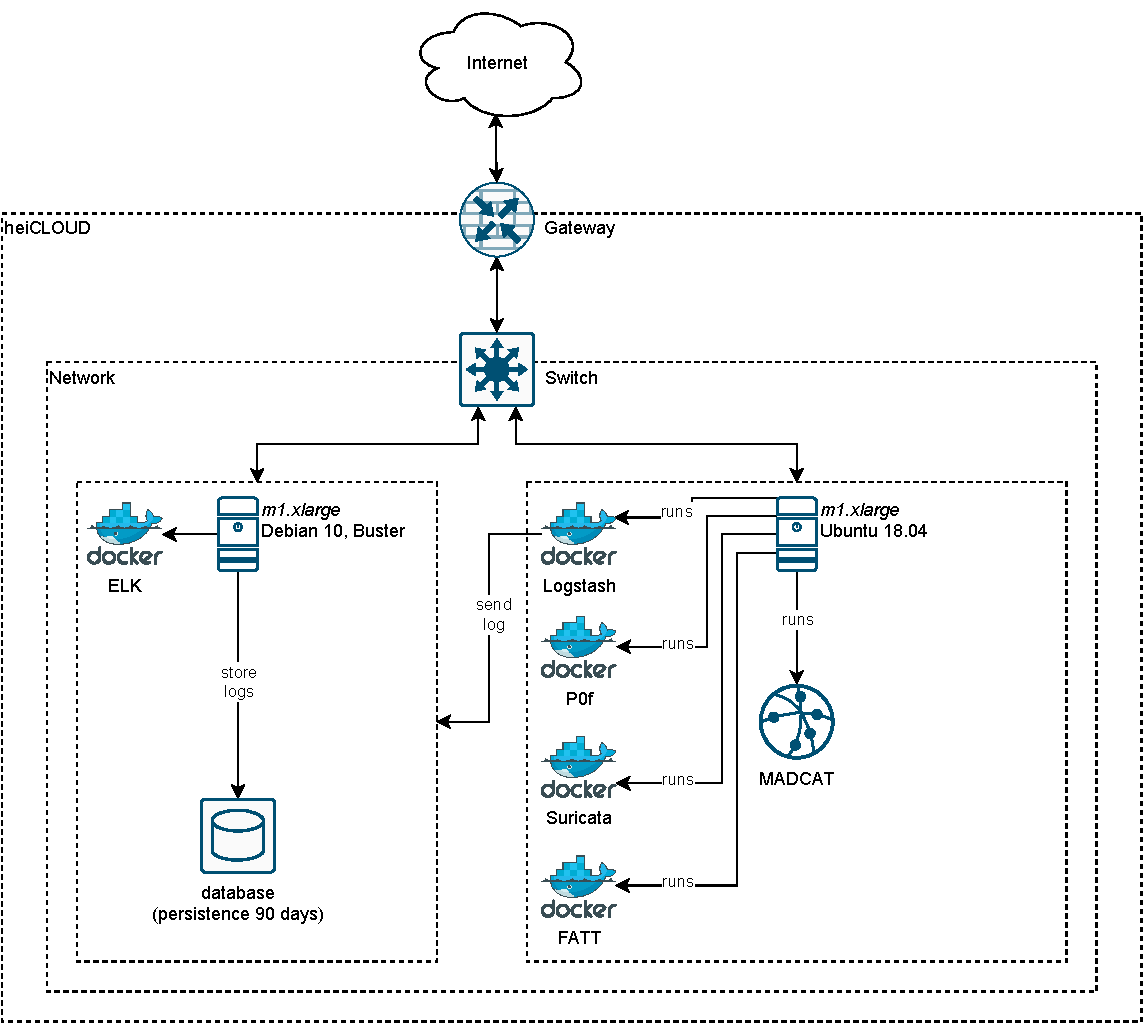
\includegraphics[width=\textwidth]{figures/heicat-conecpt.pdf}
    \caption[HeiCAT concept]{HeiCAT concept.}
    \label{fig:heicat-concept}
\end{figure}

In total, we consider three different approaches.
\begin{enumerate}
    \item heicloud
    \item Eduroam
    \item 219 Zone
\end{enumerate}

\section{Results}

\subsection{HeiCloud}

\subsection{Eduroam}

\subsection{219 Zone}
